
%(BEGIN_QUESTION)
% Copyright 2006, Tony R. Kuphaldt, released under the Creative Commons Attribution License (v 1.0)
% This means you may do almost anything with this work of mine, so long as you give me proper credit

A large water filter occasionally plugs with debris, and operations wants to have a gauge indication of this plugging.  Since plugging of the filter will result in greater differential pressure drop across it for any given amount of water flow through it, measuring pressure drop with a differential pressure gauge will provide a simple indication of filter plugging.

Draw the connecting tubes between the differential pressure gauge and the filter (the two ``taps'' shown on the pipes are ready to connect to instrument tubing) so that the gauge registers positive pressure as the filter becomes plugged:

$$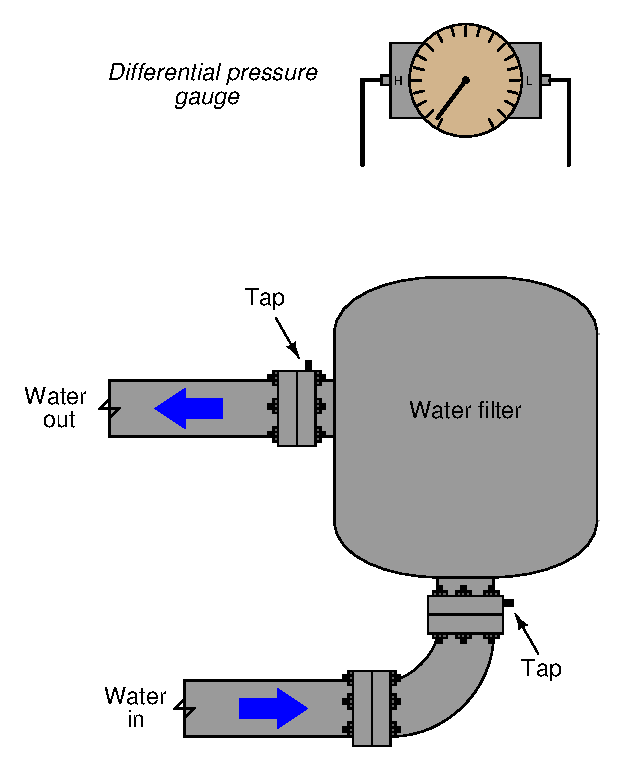
\includegraphics[width=15.5cm]{i00215x01.eps}$$

\underbar{file i00215}
%(END_QUESTION)





%(BEGIN_ANSWER)


%(END_ANSWER)





%(BEGIN_NOTES)

To properly connect this differential pressure gauge to the water filter, connect the ``high'' side to the upstream (``water in'') tap, and the ``low'' side to the downstream (``water out'') tap.

\vskip 10pt

You would choose these tap connections because the upstream side of a flow restriction will always have a greater pressure than the downstream side, and with greater plugging of the filter, you want to have greater gauge indication.  Since you want the gauge's indication to directly follow the differential pressure due to plugging, connect the ``high'' side of the gauge to the side of the filter which will develop more pressure as the plugging becomes more severe, and connect the ``low'' side of the gauge to the side of the filter which will develop less pressure as the plugging becomes more severe.

%INDEX% Measurement, pressure: using a D/P cell for filter plugging detection
%INDEX% Process: water filter (generic)

%(END_NOTES)


